% META: DONE.1

\chapterappendix{ПРИЛОЖЕНИЕ}{В}

\begin{center}
{\fontseries{sb}\selectfont Подробные схемы работы инференса}
\end{center}

\subsection{Блок-схема алгоритма работы с итоговым приложением}

На рисунке \ref{fig:app3-scheme-general} приведена общая блок-схема работы модуля.

\begin{figure}[h]
    \centering
    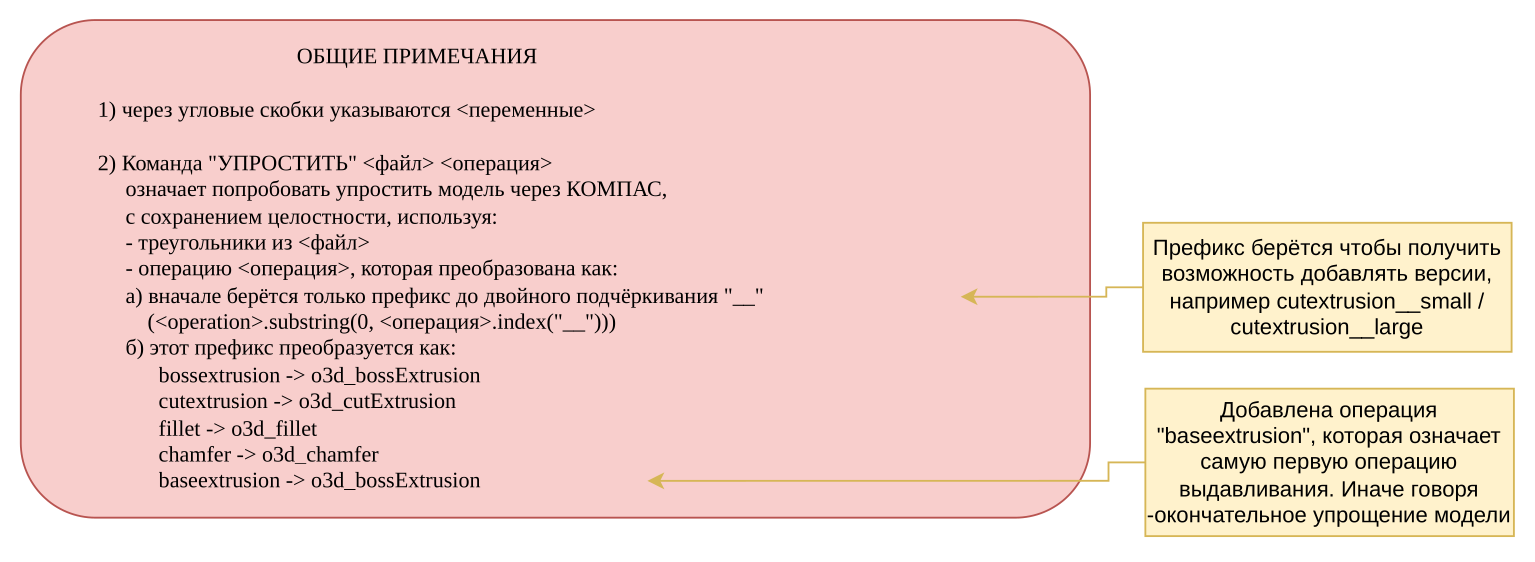
\includegraphics[width=0.8\linewidth]{figures/scheme_general.png}
    \caption{Общая схема работы}
    \label{fig:app3-scheme-general}
\end{figure}

\subsection{Автоматический режим}

На рисунке \ref{fig:app3-scheme-mode-auto} показано, как в автоматическом режиме модуль самостоятельно выбирает наиболее вероятную операцию и выполняет её сегментацию.

\begin{figure}[h]
    \centering
    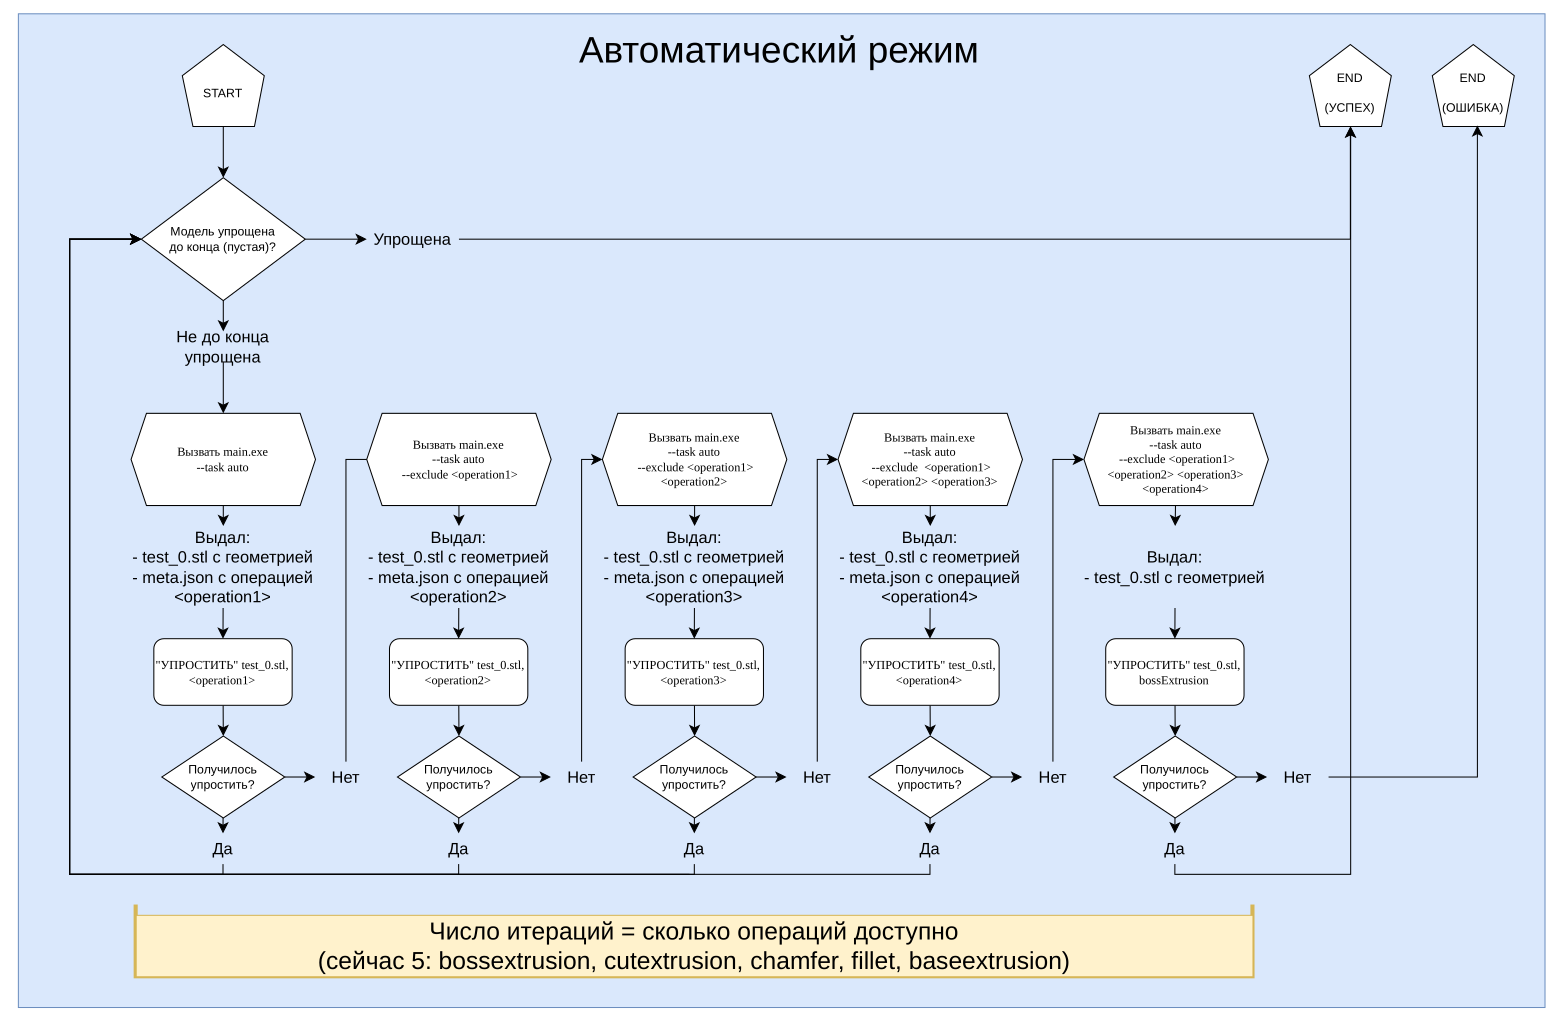
\includegraphics[width=0.8\linewidth]{figures/scheme_mode_auto.png}
    \caption{Схема автоматического режима}
    \label{fig:app3-scheme-mode-auto}
\end{figure}

\subsection{Ручной режим}

На рисунке \ref{fig:app3-scheme-mode-manual} показано, как в ручном режиме пользователь задаёт тип операции и параметры сегментации.

\begin{figure}[h]
    \centering
    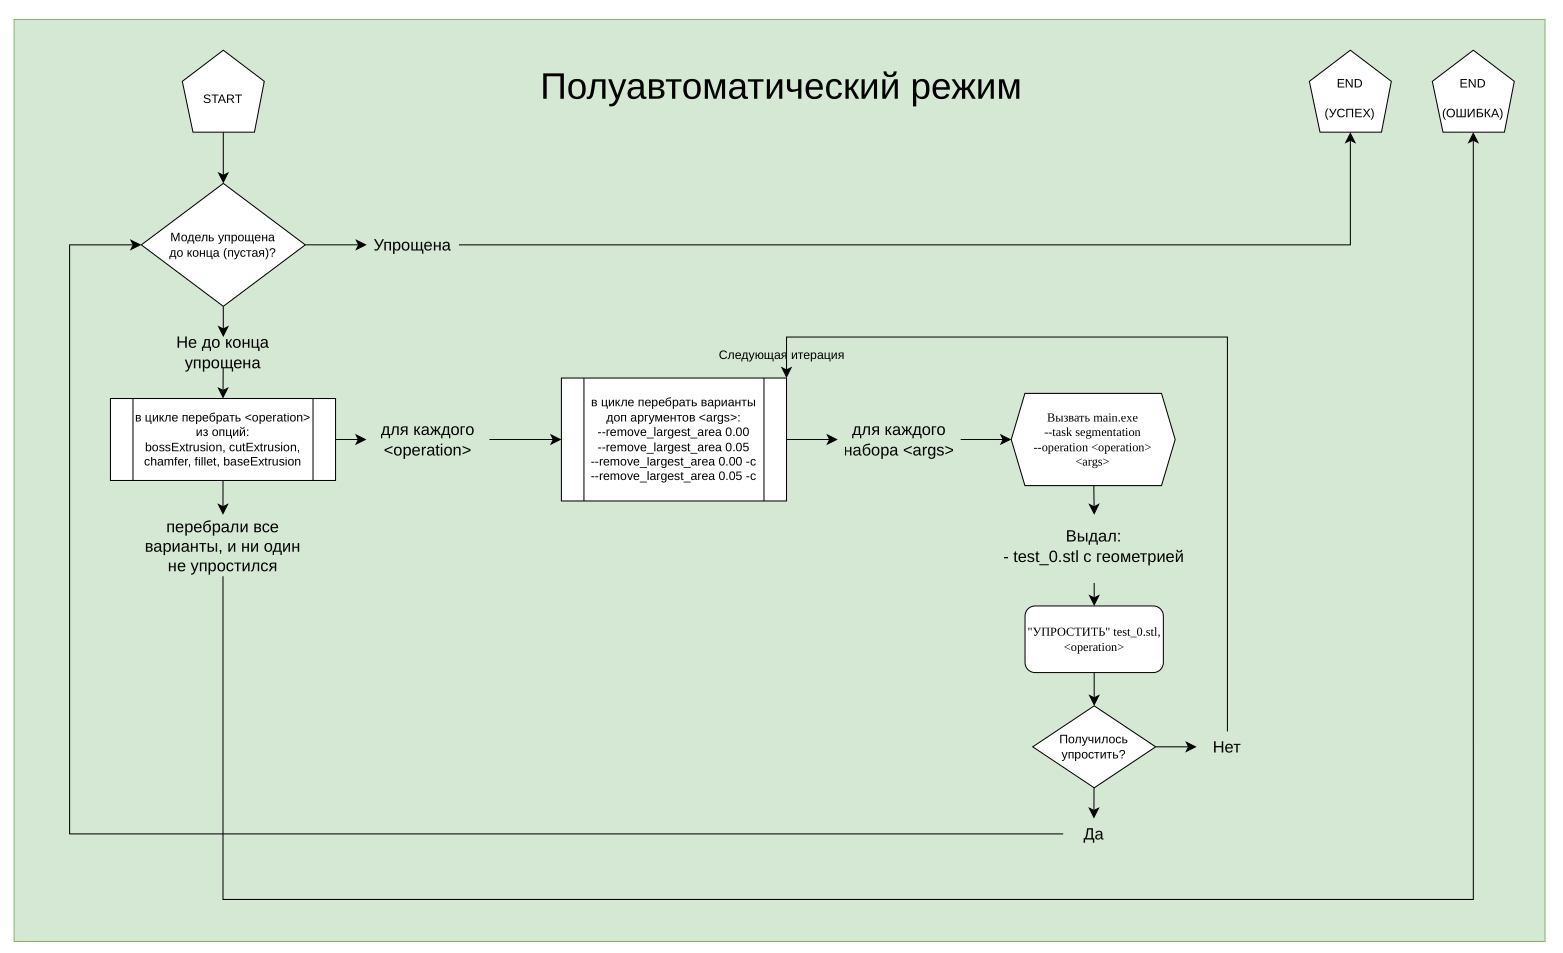
\includegraphics[width=0.8\linewidth]{figures/scheme_mode_manual.png}
    \caption{Схема ручного режима}
    \label{fig:app3-scheme-mode-manual}
\end{figure}

